\documentclass{svproc}
\usepackage[utf8]{inputenc}
\usepackage{graphicx}
\usepackage{multicol}
\usepackage{footmisc}
\usepackage{type1cm}
\usepackage{subeqnarray}
% \usepackage{natbib}
\usepackage{cite}
\usepackage{makeidx}
\usepackage{amssymb}
\usepackage{amsmath}
\usepackage{mathtools}
\usepackage{subcaption}
\usepackage{todonotes}
\usepackage{url}

\newcommand{\etal}{et al. }

\title{Applying recent machine learning approaches to accelerate the Algebraic Multigrid method for fluid simulations}
\titlerunning{Applying ML to accelerate AMG for fluid simulations}
\author{Thorben Louw \and Simon McIntosh-Smith}
\institute{
Dept. of Computer Science,
University of Bristol, 
Bristol, BS8~1UB, United~Kingdom
\email{thorben.louw.2019@bristol.ac.uk}           
\and
Dept. of Computer Science,
University of Bristol,
Bristol, BS8~1UB, United~Kingdom,
\email{S.McIntosh-Smith@bristol.ac.uk} 
}


    
\begin{document}


\maketitle



\begin{abstract}
In this work, we describe our experiences trying to apply recent machine learning (ML) advances to the Algebraic Multigrid (AMG) method to predict better prolongation (interpolation) operators and accelerate solver convergence. Published work often reports results on small, unrepresentative problems, such as 1D equations or very small computational grids. To better understand the performance of these methods on more realistic data, we create a new, reusable dataset of large, sparse matrices by leveraging the recently published Thingi10K dataset of 3D geometries, along with the FTetWild mesher for creating computational meshes  that  are  valid  for  use  in  finite  element  method  (FEM)  simulations.  We run simple 3D Navier-Stokes simulations, and capture the sparse linear systems that arise. 

We consider the integration of ML approaches with established tools and solvers that support distributed computation, such as HYPRE, but achieve little success. The only approach suitable for use with unstructured grid data involves inference against a multi-layer message-passing graph neural network, which is too memory-hungry for practical use, and we find existing frameworks to be unsuitable for efficient distributed inference. Furthermore, the model prediction times far exceed the complete solver time of traditional approaches. While our focus is on inference against trained models, we also note that retraining the proposed neural networks using our dataset remains intractable. 

We conclude that these ML approaches are not yet ready for general use, and that much more research focus is required on how efficient distributed inference against such models can be incorporated into existing HPC workflows.
\keywords{HPC-AI, AMG, GNN, Unstructured, FEM}
\end{abstract}

\section{Introduction}

In this paper, we describe our experience applying recently proposed machine learning (ML) models to predict better interpolation operators for the algebraic multigrid (AMG) method, with the aim of reducing the number of iterations the method takes to converge. Our interest lies in speeding up the solution of large, sparse linear systems which arise during fluid simulations. 

A common criticism of recent ML-based approaches to solving partial differential equations (PDEs) or accelerate scientific simulations is that they are typically demonstrated on small 1D or 2D structured grids. Yet industrial and scientific simulations currently solve problems many orders of magnitude larger, and existing tools are designed to support \textit{unstructured} 3D meshes. To be useful, ML acceleration approaches must be shown to work on these inputs. In this work, we use the 3D geometries in the Thingi10K dataset, run a simple 3D Navier-Stokes FEM fluid simulation on each, and capture the sparse matrices which result, to create a new dataset of sparse linear systems for evaluating such ML approaches.

In 2020, Luz \etal reported using a graph neural network (GNN) approach for accelerating AMG that is able to deal with unstructured data~\cite{Luz2020}. Since they found good generalization to domains outside of their original training regime, we use their implementation as a basis for our work.

Machine learning models such as the one in \cite{Luz2020} learn good values for parameters in a process called \textit{training}. Training is much more computationally demanding than \textit{inference} against a trained model, so it attracts the bulk of research attention today. However, the researcher wanting to use or deploy a trained model for inference is left with a significant amount of software engineering effort to make their model to run well, and this is not often discussed. 

A disconnect exists between the way high-performance computing (HPC) tools are designed to scale in over the distributed compute nodes in a supercomputer, which typically using implementations of the Message Passing Interface (MPI) to communicate over fast interconnects and are invoked via workload managers such as Slurm, and the support for serving machine learning models in the dominant ML frameworks, which favor a cloud-like distributed computing setup. Model serving frameworks load trained, optimized models and make them available to clients through an interface such as gRPC. They optimize for latency and throughput, dynamically batching requests and scaling compute resources to match demand, and allow optimized models to make use of acceleration hardware, using hardware-specific frameworks such as NVIDIA's TensorRT that optimizes models to make use of  TensorCores on NVIDIA accelerators. Alternatively, one might wish to simply load a model locally in an application by integrating modern machine learning frameworks directly in source code. Even so, the post-training optimization process can involve serializing to a model interchange format like ONNX \cite{onnx}, sparsification, data-type reduction and quantization, and running models through deep learning (DL) compilers such as TVM~\cite{TVM} to optimize computation and data movement. This difficulty is reflected in the growth of a software engineering trend called ``MLOps'' (Machine Learning Operations), which recognizes that the devising and training models is only a small part of the overall effort in making these models useful~\cite{paleyes2020challenges, konstantinos2020ml}.

Our attempt at using the approach in \cite{Luz2020} with our dataset fails: the message-passing graph neural network (GNN) model, and the graph neural network framework used for the implementation do not scale to support the size of matrices in our dataset. An inference against the model -- one small part of the problem setup phase -- runs longer than a traditional solver takes to complete the whole solution, and uses huge amounts of memory even for modest problem sizes. In addition, the model does not generalize well to even the smaller sparse matrices in our dataset. We find that support for distributed exact inference using large graphs in GNN frameworks today is limited, and difficult to integrate into our workflow. The GNN nature of the model makes it difficult to optimize, and support in the common ONNX interchange format is lacking.

The structure of the rest of this paper is as follows, we give an overview of AMG in Section \ref{sec:amg} and discuss our evaluation dataset in Section~\ref{sec:dataset}. We review of the recently proposed ML acceleration approaches for AMG in Section~\ref{sec:ml-methods} with special focus on the approaches of Greenfeld \etal \cite{Greenfeld2019} and Luz \etal \cite{Luz2020}. We discuss our results in Section~\ref{sec:results} before concluding with some thoughts on future work.

%  interchange format such as ONNX~\cite{onnx}, model sparsification~\cite{ashouri2018fast, kurtz2020inducing}, data-type reduction and quantization, and running models through deep learning compilers such as TVM~\cite{TVM} 


% Modern ML frameworks already incorporate many thousands of hours of work for model optimization (XLA, MLIR, graph compilation, kernel fusion, optimized kernels for operations), which we do not want to re-use.

%Sufficiently large neural networks trained with enough representative data can generalize to cope with very wide range of input distributions and be adapted for a variety of tasks. An extreme recent example is the GPT-3 language model~\cite{gpt3} with 175 billion trainable parameters, trained on hundreds of billions of input samples. But it can be fine-tuned for task-specific applications using only thousands of new examples. However training GPT-3 has been estimated between 4 and 13 million US dollars. 

Our contributions in this work are
\begin{itemize}
    \item A new dataset of 30,000 sparse linear systems representative of
    the fluid mechanics arising on FEM on complex 3D geometries. The dataset is easy to modify for different problems and boundary conditions, and useful for practically evaluating suggestions for ML-accelerated solvers.
    \item Findings from our experience with the model from Greenfeld \etal~\cite{Greenfeld2019}, which demonstrate that much simpler models can also learn good interpolation operators, with corresponding benefits for integrating them into applications 
    \item A description of our experience trying to apply a Graph Neural Network such as the one in~\cite{Luz2020} to larger, 3D fluid dynamics problems.
    
\end{itemize}


\section{Background}
\subsection{Overview of Algebraic Multigrid}
\label{sec:amg}
In this section we give a very brief the AMG concepts which are important for contextualizing the ML methods which follow. A thorough overview of AMG is available in~\cite{STUBEN2001281}.

In this setting, we are interested in solving linear systems of the familiar form:

\begin{equation}
A\mathbf{x} = \mathbf{b}
\end{equation}

where $A \in \mathbb{R}^{n\times n}$ is a very sparse matrix. These systems frequently arise in scientific domains when solving partial differential equations (PDEs) that are discretized on a computational grid, and then solved using techniques such as FEM, or the Finite Difference Method (FDM) or Finite Volume Method (FVM) For example, in a typical fluid dynamics solver, such linear systems are solved at each timestep when calculating the next grid values for the velocity and pressure fields.

In real-world problems these linear systems are both very large (many millions of rows), and extremely sparse, encouraging the use of specialized solvers which take advantage of these properties. Iterative \textit{relaxation} methods are used, which improve on an initial guess until the solution converges (i.e. until the residual $e_i = \| A\mathbf{x}_i - \mathbf{b}\|$ becomes sufficiently small).

Many relaxation methods have been developed over the last few decades, including the well-known class of Krylov subspace methods such as the Conjugate Gradient (CG) method and Generalized Minimal Residual Method (GMRES).

Relaxation methods are known to be good at reducing high-frequency errors (associated with eigenvectors of $A$ that have large eigenvalues), but poor at reducing the smooth or low-frequency errors, and can need many iterations to converge.

Multigrid methods improve on this situation by creating a hierarchy of coarser (smaller) grid levels. At each level, residual errors after applying smoothing at the fine grid level are projected to the next coarsest grid using a problem- and level-specific `restriction operator' $R$, before applying smoothing (relaxation) at the coarser grid level. This process is repeated, resulting in smaller and smaller linear systems, until eventually a system is small enough to solve directly. The coarsest grid error is then interpolated back from coarse to fine grid levels using problem- and level-specific `prolongation operators' $P$ and added back to the post-smoothing guess as a correction, until finally a few relaxations are applied to the finest system. This entire process forms one ``V-cycle'', several iterations of which are performed until the residual converges.

Coarse-grid correction smooths out the low-frequency errors, while relaxations at the finest grid level smooth out the high-frequency errors, resulting in rapid convergence ($O(n)$ iterations for a grid with $n$ nodes, in the optimal geometric multigrid case).

In the original Geometric Multigrid context, the problem geometry (`grid') is available to the solver, but the Algebraic Multigrid method~\cite{AMGorginal} extends this multilevel idea to general linear systems in a `black-box' fashion, using only the entries of the matrix $A$ and the target vector $\mathbf{b}$ as inputs. Coarsening strategies in AMG use algebraic properties of the nodes in the matrix (such as the strength-of-connection or energy-based properties) rather than the problem geometry to select coarse nodes, and heuristic methods to select the weights in the prolongation operator. 

AMG's black-box approach may be less efficient than approaches which can exploit the problem geometry, but it has an important software engineering advantage: easily re-usable, optimized libraries for the solution of general linear systems from different domains using can be created which use standard matrix-vector interfaces. Examples of such libraries in the HPC world are HYPRE's BoomerAMG solver~\cite{hypre} and ML~\cite{ml-guide}, which have developed parallel versions of AMG algorithms that support distributed sparse matrices for very large systems, and scale well over thousands of nodes. 

\paragraph{Coarsening strategies}
Several algorithms have been proposed to identify which nodes of the grid are ``coarse'' (to be included in the next grid level), and which are ``fine''. This split is used to create the next grid level, but also forms vital information in the construction of the operators which interpolate values back between the coarse and fine grids.

Examples are the ``classical'' Ruge-St\"uben coarsening~\cite{AMGorginal}, Cleary-Luby-Jones-Plassman (CLJP)~\cite{cleary1998coarse}, and parallel coarsenings which lead to lower operator complexity, such as Parallel Modified Independent Set (PMIS) and HMIS~\cite{de2006reducing}. The aggressiveness of the coarsening influences the size of the next-coarsest grid (and thus the run-time of the final algorithm), but also impacts the subsequent choice of interpolation operators.

\paragraph{Interpolation and the construction of the Prolongation operator}
Between two grid levels, the error propagation matrix is given by
\begin{equation}
\label{eq:error-matrix}
M = S^{\sigma_2}(I - P[P^TAP]^{-1}P^TA)S^{\sigma_1}
\end{equation}

where the $S$ terms represent error propagation matrices of the pre- and post-smoothing relaxation sweeps.

The asymptotic convergence rate of AMG is determined by the spectral radius of this error propagation matrix $\rho(M)$. After the the pre- and post-smoother are chosen, $\rho(M)$ depends only on $P$. While a good $P$ is one that results in a small spectral radius for $M$, it should also be sparse for computational efficiency.

% The classical ``direct'' Ruge-St\"uben interpolation heuristic~\cite{ruge1987algebraic} uses weights according to the formula:
% \begin{equation}
% \label{eq:classical-weights}
% w_{ij} = -\dfrac{
% a_{ij} + \sum\limits_{m \in D_i^s}\left(\dfrac{
%     a_{im}a_{mj}
% }{
%         \sum\limits_{k \in C_i}a_{mk}}\right)
% }{
%     a_{ii} + \sum\limits_{n \in D_i^w
%     }a_{in}
%     }
% \end{equation}

% where $D^w_i$ is the set of weakly-connected fine nodes, $D^s_i$ is the set of strongly-connected fine nodes, and $C_i$ is the set of coarse nodes in the immediate (distance~1) neighborhood of the node $i$ (and the ``strength of connection'' criterion is defined algebraically)~\cite{stuben2000algebraic}. The rows of $P$ are constructed such that if the $i$th node is coarse, the $i$th row will be identity, else the weights from Equation~\ref{eq:classical-weights} are used.

% Other prolongation strategies have been proposed, such as Jacobi and multi-pass interpolation, as well as truncating the interpolation to promote sparsity in $P$~\cite{stuben2000algebraic}.

We note that the restriction operator which maps from fine to coarse grids is usually chosen such that $R = P^{T}$.

The methods we consider in Section~\ref{sec:ml-methods} aim to improve on the weights in a candidate $P$.


\paragraph{Use of AMG as a preconditioner}
The multilevel nature of AMG means that each iteration is much more expensive to execute than an iteration of a single-level Krylov solver. As a result, instead of being used as a standalone solver, AMG is frequently used as a preconditioner to improve the convergence of Krylov subspace methods. In this task, only a few AMG iterations are run to get an approximate solution, and the setup cost of AMG (including building $P$) becomes more important than the cost of AMG iterations to solve the system.

\subsection{A dataset of sparse systems from 3D unstructured meshes}
\label{sec:dataset}
To evaluate the usefulness of newly proposed methods, we build a large dataset of sparse matrices captured from simple FEM fluid simulations on a diverse set of geometries. Our search for existing open datasets of geometries to leverage as a starting point led us to Zhou and Jacobson's 2016 Thingi10K dataset~\cite{zhou2016thingi10k}, which contains 10,000 3D printing models. Similar sources of 3D shape datasets exist in the ModelNet~\cite{modelnet} and ShapeNet~\cite{chang2015shapenet} datasets. However, Thingi10K was chosen since it has already been used as an evaluation set for the  FTetWild mesher~\cite{ftetwild}, which transforms ``triangle soup'' input meshes into high quality tetrahedral meshes that are valid for use with FEM simulations.

To generate our dataset, we use the FEniCS~\cite{fenics} framework with the 10,000 high quality versions of the Thingi10K meshes after FTetWild processing, and implement a simple 3D Navier-Stokes simulation using P2-P1 (Taylor-Hood) finite elements with a time-varying pressure condition, and Dirichlet boundary conditions. At each timestep, the solver must solve three large linear systems representing the velocity update, pressure correction, and velocity correction steps. After a few timesteps, we capture these linear systems to files, giving us 30,000 test matrices. 

This process could be re-run with a variety of boundary and initial conditions, different PDEs with various coefficients, different FTetWild triangle densities, and different solvers (e.g. finite volume method simulations) to easily generate many other candidate sparse linear systems to evaluate the accuracy of acceleration methods.

An example of a mesh from the Thingi10K dataset is shown in Figure~\ref{fig:data-viz}. Here we show Item 47251 (``Living Brain Right Part''). The geometry is transformed using FTetWild then used as the basis for a simple FEM simulation with 438,897 degrees of freedom. We show a rendering of the original mesh (252,204 faces), and a visualization of the corresponding sparse matrix from the velocity update step of our simulation. The square matrix is challenging at 2,995,242 rows, but is also 99.997\% sparse. While this is still orders of magnitude smaller than problem sizes in industrial applications, it is more representative of the problems we wish to solve than the small test problems used in~\cite{Luz2020} (64 -- 400,000 rows).

\begin{figure}
    \centering
  \begin{subfigure}{.5\textwidth}
  \centering
    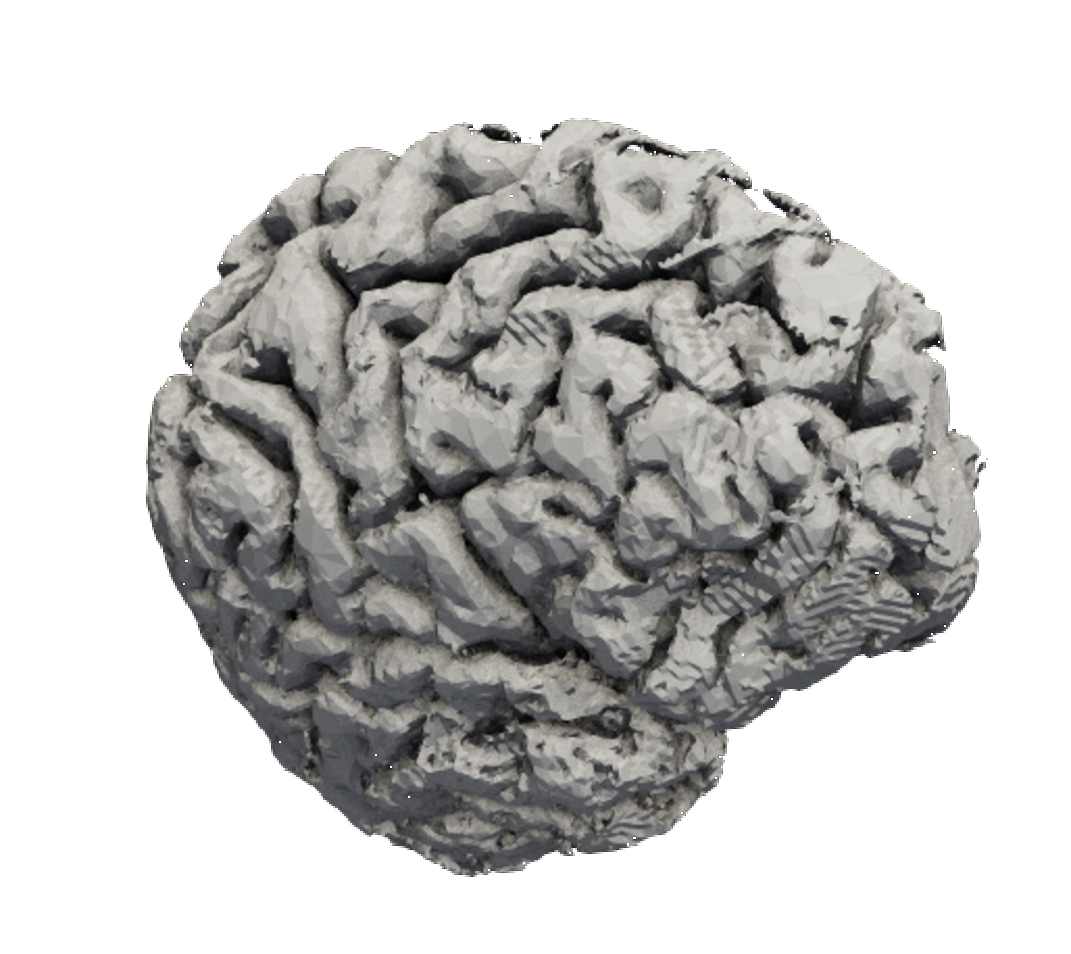
\includegraphics[width=0.8\linewidth]{images/brain2.pdf}
  \caption{Rendering of the mesh geometry}
  \label{fig:rendering-mesh-geom}
\end{subfigure}%
\begin{subfigure}{.5\textwidth}
  \centering
  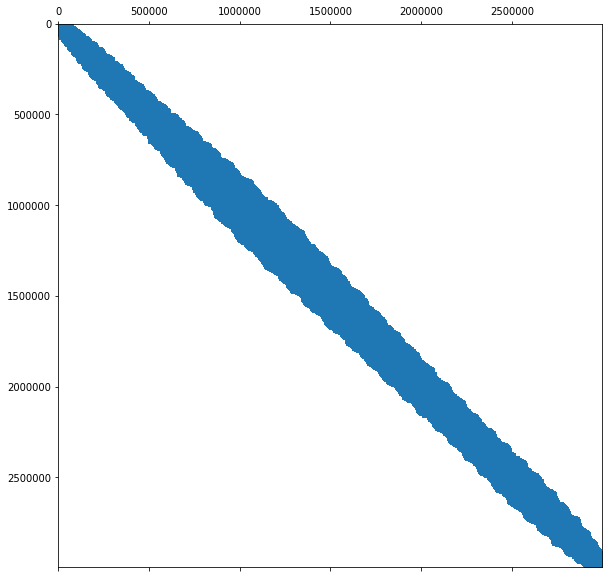
\includegraphics[width=.9\linewidth]{images/sparse-matrix.png}
  \caption{Corresponding sparse matrix }
  \label{fig:sparse-matrix-of-brain}
\end{subfigure}
\caption{Item 47251 \textit{Living Brain Right Part} from the Thingi10K dataset, with a visualisation of the corresponding sparse matrix from a FEM fluid simulation using this geometry.}
\label{fig:data-viz} 
\end{figure}


Figure~\ref{fig:data-set-characteristics} gives an overview of the matrix sizes and sparsity of the the matrices in the dataset (default FTetWild triangle density). As we will discuss in Section~\ref{sec:luz}, the sparse matrices are also much larger than those used in benchmark datasets for common graph neural network frameworks.

\begin{figure}
    \centering
  \begin{subfigure}{.5\textwidth}
  \centering
    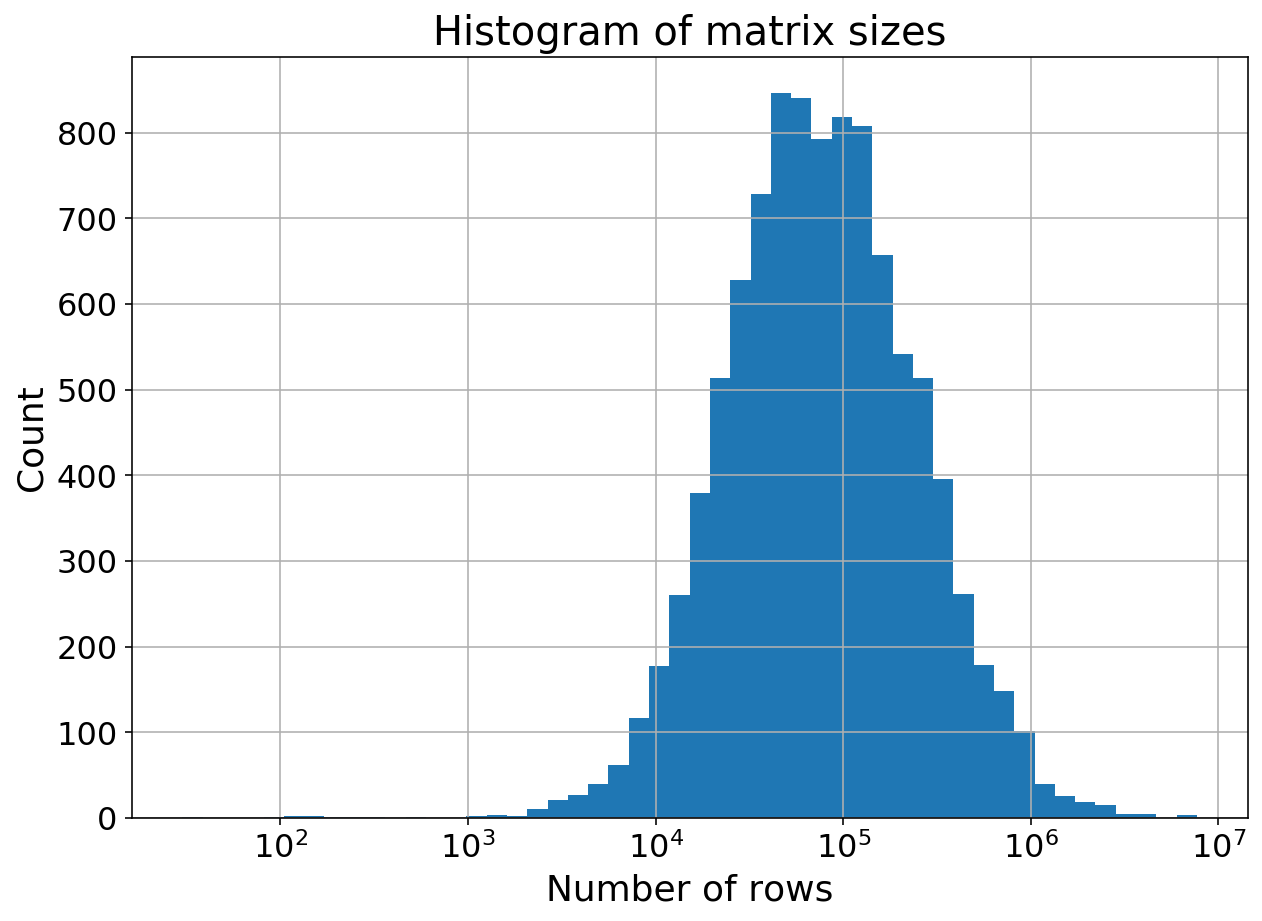
\includegraphics[width=0.97\linewidth]{images/matrix_sizes.png}
  \caption{Distribution of matrix sizes }
  \label{fig:sub1}
\end{subfigure}%
\begin{subfigure}{.5\textwidth}
  \centering
  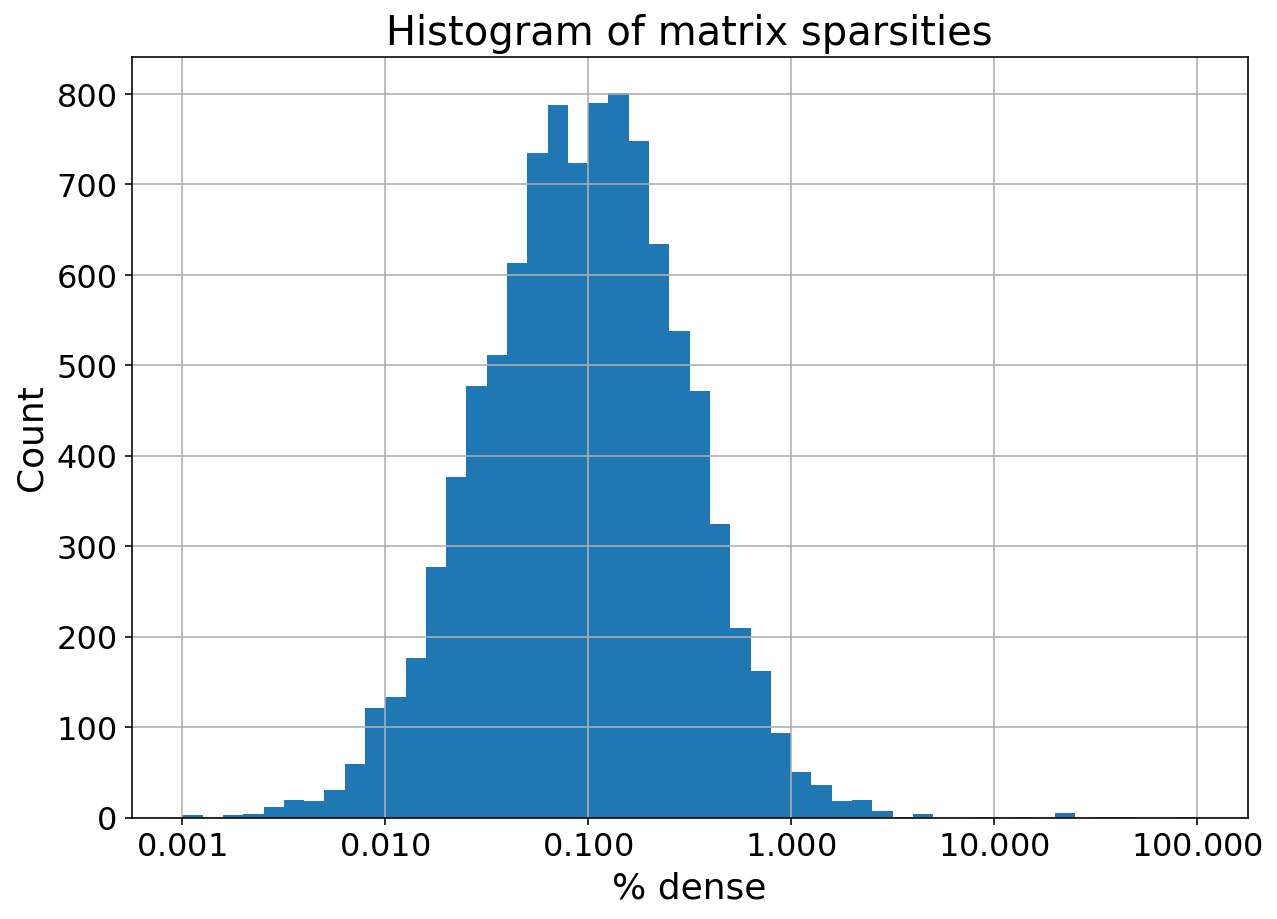
\includegraphics[width=.97\linewidth]{images/matrix_sparsities.png}
  \caption{Distribution of matrix sparsities }
  \label{fig:sub2}
\end{subfigure}
\caption{Distribution of matrix sizes and sparsities in the dataset (velocity projection step only)}
\label{fig:data-set-characteristics} 
\end{figure}


% How does this compare with other matrices? SuiteSparse (https://sparse.tamu.edu/) has fewer than 200 matrices marked `fluid' and not necessarily suitable, https:/ /snap.stanford.edu/data/ has data used in Graph problems.

% Crucially, the classical Ruge-Stuben solver is not guaranteed to converge for these systems. In fact, only TODO percent of them converged. But we could be e.g. Krylov acceleration and other interpolation (extended+i) and coarsening strategies (PMIS).

\section{Overview of the recently proposed methods}
\label{sec:ml-methods}
The earliest work we are aware of which tries to predict better prolongation operators for AMG using machine learning is the Deep Multigrid Method proposed by Katrutsa, Daulbaev and Oseledets~\cite{Katrutsa2017}, which they demonstrate only on small structured grid problems for PDEs in 1D. The method is not practical because it requires training a new deep neural network for every new matrix $A$. We did not apply it in our work.

For our work, we were specifically attracted to the approaches in Luz \etal~\cite{Luz2020} and the work preceding it in Greenfeld \etal~\cite{Greenfeld2019}, which try improving on the values in a candidate $P$ produced by some existing method. Since methods use previously computed coarsening and prolongation sparsities, they can leverage the decades of work in existing AMG solvers.

% Although the two papers we discuss below differ significantly in their applicability, neural network design choices and choice of inputs, they both recast the problem of predicting the values of $P$ as a learning problem, where the aim is to minimize the spectral loss of the error matrix $\rho(M)$ (Equation~\ref{eq:error-matrix}). 
\paragraph{Learning to minimize $\rho(M)$}
In all three of these works, the problem of predicting a good $P$ is recast as a learning problem where the aim is to minimize $\rho(M)$, the spectral radius of the two-grid error matrix from Equation~\ref{eq:error-matrix}. 

Any algorithm that tries to minimise $\rho(M)$ directly faces a difficult time: evaluating $\rho(M)$ means inverting the large $(P^TAP)^{-1}$ term in Equation~\ref{eq:error-matrix}, and subsequently performing a very expensive ($\mathcal{O}(n^3)$) eigen-decomposition with $n$ extremely large. To make matters worse, neither TensorFlow nor PyTorch (the two most popular DL frameworks) currently support sparse matrix inversion, and converting to dense representations is infeasible for problems of this size.

Instead, Katrutsa, Daulbaev and Oseledets~\cite{Katrutsa2017} approximate the spectral radius using Gelfand's formula, and develop an efficient, unbiased stochastic estimator for this approximation. It still requires evaluating norms of $M$, and thus computing the expensive $(P^TAP)^{-1}$ term.

In contrast, both~\cite{Luz2020} and~\cite{Greenfeld2019} choose a proxy loss function: they minimize the upper bound for the spectral radius given by the Frobenius norm $\|M\|^2_{F}$. To avoid the large cost of evaluating the $(P^TAP)^{-1}$ term directly, they restrict their training data distribution to specially synthesized block-circulant, block-diagonalized matrices, where the norm is the sum of the small diagonal blocks' norms. This allows efficient and stable calculation of the loss function, but restricts the distribution of input matrices available for training.

\subsection{Deep residual feed-forward network for 2D structured grid problems (Greenfeld \etal~\cite{Greenfeld2019})}
\label{sec:greenfeld}
Our interest is in methods that work for 3D \textit{unstructured} grids, but in this section we briefly discuss the work of Greenfeld \etal~\cite{Greenfeld2019}. Their neural network model is for a 2D structured grid discretized using a $3\times 3$ stencil. However, it lays important groundwork for the unstructured grid method which follows.

\paragraph{Input and output}
The proposed deep neural network aims to improve on values in a candidate prolongation matrix as determined by an existing interpolation algorithm, by only using information local to each coarse point. The same network is used to to predict $P$ at all levels of the grid.

In addition to inference against the model, there is non-trivial pre- and post-processing to assemble the inputs and interpret the neural network's outputs.

As input, for each coarse point in the grid, we pass to the network the equivalent point in the fine grid and its four nearest neighbors, using the $3 \times 3$ stencil of each of these 5 points, resulting in 45 real values which are concatenated and flattened to build an input in $\mathbb{R}^{45}$. 

The output of the network is fixed to be in $\mathbb{R}^4$ and represents the weightings of the coarse point to the fine grid points to the north, south, east and west. Remaining directions' weightings are then solved algebraically. In the specific problem formulation the authors choose, the sparsity of the columns in $P$ is fixed to allow at most 9 non-zeros, and the maximum distance to which coarse points can contribute to fine points is fixed at 1.

Despite its limitations, this network is more flexible than earlier proposals for PDE solvers such as the one in Tang~\cite{Tang2017}: it works for grids of any size without re-training, as long as the stencil size of the problem is the same. The authors also show some generalization capability when used with different boundary conditions and distributions of coefficients for the underlying PDE. 

However, this approach involves very tight integration with the problem being solved, and means training entirely different networks for different discretizations (consider that when using a 3D 27-point stencil instead of a 2D 9-point stencil, the concatenated, flattened inputs will be in $\mathbb{R}^{189}$ instead of than $\mathbb{R}^{45}$), and needs an entirely different formulation to use longer-range interpolation strategies. It is also limited to structured grids, so we look to another proposal to tackle the unstructured problems of interest in our dataset.


\subsection{Graph neural networks for unstructured problems (Luz \etal~\cite{Luz2020})}
\label{sec:luz}
Seeking to extend the work of Greenfeld \etal to unstructured problems, Luz \etal develop an approach in~\cite{Luz2020} which uses the Graph Neural Network shown in Figure~\ref{fig:gnn}. 

\begin{figure}
    \centering
    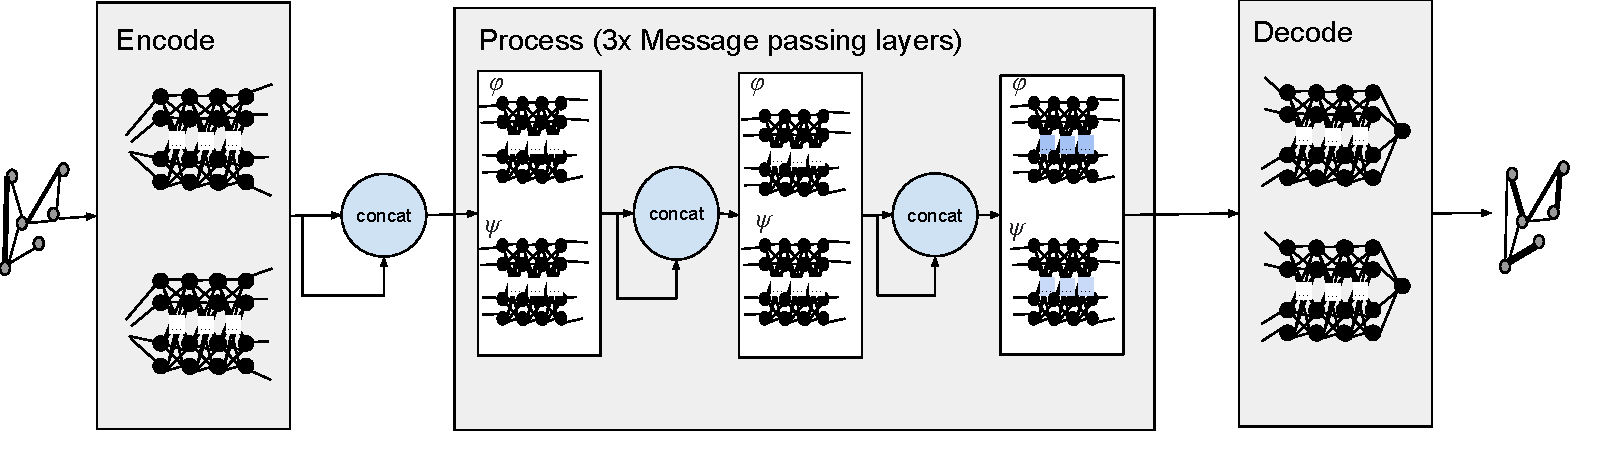
\includegraphics[width=\linewidth]{images/GraphNeuralNet.pdf}
    \caption{The graph neural net used in~\cite{Luz2020}.}
    \label{fig:gnn}
\end{figure}

GNNs are a recent kind of machine learning model that can deal with general unstructured input. A common unifying framework for reasoning about graph networks is presented by Bataglia \etal in~\cite{battaglia2018relational}, who also developed the DeepMind GraphNets library that Luz \etal used for the implementation of this model.

Luz \etal learn to predict $P$ using a non-recurrent encode-process-decode architecture, in which
\begin{itemize}
    \item the \textit{encode} block learns a representation of the input edge and node features in a higher-dimensional latent space ($\mathbb{R}^{64})$. It has two 4-layer dense feed-forward neural networks to learn this function for edges and nodes independently.
    \item the \textit{process} block consists of 3 message-passing layers. In graph networks, message passing layers (Gilmer \etal~\cite{gilmer2017neural}) are a graph generalization of spatial convolution, and are essential for learning representations. Message passing layers produce a ``message'' for each edge by evaluating some learned function $\phi$, taking as input the edge feature and the node features of the edge's incident nodes. Then, for each node, we aggregate the messages from its edges using another learned function $\psi$ which takes as input the sum reduction of the incoming messages. In graph neural networks, the learnable functions $\phi$ and $\psi$ are implemented using some choice of neural network. Luz, \etal use 4-layer dense feed-forward networks, but also choose to concatenate each message layer's input with the previous layer's input\footnote{We find that a bug in the authors' implementation also concatenates the encoded input with itself before being fed to the message passing layers}.
    \item the \textit{decode} block translates the high-dimensional latent node and edge representations back into a single real value per edge using two independent 4-layer feed-forward networks.
\end{itemize}

This model has 286,146 learnable parameters.

In addition to the model, there are non-trivial pre-processing and post-processing tasks to translate between the sparse tensors in the problem domain and the data structure (a ``GraphsTuple'') used by the GraphNets framework. 

Similar to the Greenfeld \etal model in~\ref{sec:greenfeld}, to prepare the input to the network, we need the list of coarse nodes from an existing coarsening method, a candidate prolongation matrix from an existing method, and the sparse matrix $A$. These are transformed into a GraphsTuple structure in which nodes are one-hot encoded to indicate whether they are coarse or fine, and edge values are concatenated with a one-hot encoding indicating whether they are included in the candidate $P$'s sparsity pattern. Note that the size of the graph structure depends on both the size and the sparsity of $A$.

The output from the graph network is another GraphsTuple, from which the final $P$ must be reconstructed. The original coarse nodes list is used to select the columns of $P$, and the baseline $P$ is used to re-impose the sparsity pattern (i.e. only selecting those edge values from the graph network output). 

The current implementation uses the DeepMind GraphNets library, which in turn is based on the Sonnet library that builds on the well-known TensorFlow ML framework, allowing the implementation to use TensorFlow's optimised kernels for sparse and dense Tensor operations on various devices, and benefiting from TensorFlow's extensive ecosystem of tooling. However, we note that other graph network libraries exist which are more actively maintained and report better performance, such as DGL~\cite{DGL}.



\section{Results}
\label{sec:results}
\subsection{For the model in Greenfeld \etal}

\paragraph{Faster training with simpler models}
The authors of~\cite{Greenfeld2019} choose a 100-wide, 100-deep residual feed-forward network with over $10^6$ trainable parameters to learn the $f:\mathbb{R}^{45} \rightarrow \mathbb{R}^4$ mapping, without justifying why such an expressive network might be necessary (although they state in their conclusions that future work should consider simpler models). The network as proposed in~\cite{Greenfeld2019} took almost a day to train on a high-end (Intel Xeon 8168 48-core) CPU, or several hours on a GPU -- a prohibitive upfront cost for a method so tightly integrated with the specific problem being solved, considering that the problem sizes in~\cite{Greenfeld2019} only take seconds to solve using a traditional solver.

%\footnote{A residual network includes feedforward skip connections that pass the output of a layer directly to another layer much deeper in the network. This technique has been shown to stabilize vanishing gradients during training, enabling much deeper neural networks~\cite{resnet}. } 

Pursuing simpler, shallower neural network models is attractive because they would not only allow for a faster forward pass and much less computation during inference, but also consume less memory, and require fewer weights to be loaded from a serialized description of the model.

We retrained two much simpler network architectures: a simple 4-layer encoder-decoder network (layer widths 100, 50, 30, 50 with ReLu activations) with 12,998 learnable parameters and a shallow 2-layer multi-layer perceptron (layer widths 20, 10 with ReLu activations) with 1,038 learnable parameters. Layer widths were chosen to result in networks with approximately two and three orders of magnitude fewer learnable parameters than that proposed in \cite{Greenfeld2019}, respectively. 

Informed by results showing that incorporating large learning rates aids rapid learning convergence (Wilson \etal~\cite{wilson2017marginal}), we also introduced an exponentially decaying learning rate schedule with a large initial value ($\epsilon=0.1$, decay rate $0.95$) to replace the authors' approach of only setting a small initial learning rate ($\epsilon=1.2 \times 10^{-5}$). When used with the common ``early-stopping'' technique~\cite{prechelt1998early}, these changes can reduce training from hours to minutes on a CPU, yet we still achieve very good prediction accuracy. The simple networks continue to outperform the classical Ruge-St\"uben interpolation the authors of~\cite{Greenfeld2019} use as a baseline comparison, although not as well as the original network, and the simplest network's results do not generalize to larger matrix sizes (see Table~\ref{tab:simpler-nn-results}).

\begin{table}[]
    \caption{Performance of simpler network architectures applied to the work in~\cite{Greenfeld2019}, indicating the percentage of cases where the model's predicted $P$ resulted in convergence in fewer V-cycle iterations of AMG to solve the 2D FEM problem than a baseline Ruge-St\"uben solver}
    \centering
    \begin{tabular}{c c c c}
         Grid size &  Original from~\cite{Greenfeld2019} & \hspace{3mm} 4 layer enc-dec & \hspace{3mm} 2-layer MLP\\ \hline
         32x32 & 83\% & 93\% & 96\% \\         
         64x64 & 92\%  & 90\% & 88\%\\         
         128x128 & 91\% & 88\% & 78\% \\
         256x256 & 84\% &   82\% & 78\%\\
         512x512&  81\% & 86\%   & 68\%\\
         1024x1024&  83\% & 80\% & 52\%
    \end{tabular}
    \label{tab:simpler-nn-results}
\end{table}

\paragraph{Integration and parallelization}
The design of the model in~\cite{Greenfeld2019} allows it to be used in a parallel, distributed-memory setting. Gathering the stencil of surrounding nodes uses mostly local values and communication patterns very similar to those required during coarsening and classical interpolation, and allows extensive re-use of values already in a distributed node's memory. Similarly, since the network considers each input in isolation, it is possible to have several distributed instances of the model to query (possibly one per node), and we can batch inputs to the network for efficient computation. Finally, the simplest network we found has a very light computational profile (two layers of matrix multiplication and activation function computation) and not many weights to load during model deserialization, making it feasible to use the model on the same nodes where the coarsening and interpolation work happen. Models are agnostic to the size of the input grid, making them re-usable. Even though a different model may be needed for each problem (distribution, boundary conditions), having pre-trained model weights for a variety of problem settings available for download in a `model zoo' might be feasible.

% Assembling the graph input can be done in parallel?

% This ability to integrate with existing methods (and those amenable to parallelisation), is an appealing property of both the Luz \etal, and Greenfeld \etal approaches.


\subsection{For the model in Luz \etal}
\paragraph{Scalability of inference}
First, we try to evaluate how well a model trained as described in~\cite{Luz2020} could cope with the matrices in our dataset without modification.

A problem quickly becomes apparent: as shown in Figure~\ref{fig:small-runtime-inference}, when performing inference on a single node, the execution time of the forward pass of the graph network quickly becomes problematic for larger matrices, e.g. taking almost 5 min for a medium-sized $800,445\times800,445$ matrix in our test set on a 48-core Intel Skylake CPU. This inference represents only the first level of the grid's setup of $P$ -- in a real problem setting, subsequent levels still would need to make inferences in serial (for progressively smaller graphs) during the problem setup phase. For comparison the single-core pyAMG \cite{pyamg} solver using a classical direct framework for this same problem takes just 71.1s for the whole problem setup phase and 50.5s for the iterations, i.e. the traditional approach using a single core can solve the whole system in less time than just a small portion of the setup phase takes using the GNN model.

The time complexity of the GNN inference is linear in the size of the input network. Wu~\cite{wu2020comprehensive} derives the time complexity of similar message-passing Graph Convolutinal Network (GCN) layers as $\mathcal{O}(Kmd + Knd^2)$ with $K$ the number of layers in the network, $m$ the number of edges and $n$ the number of nodes $d$ is a fixed constant denoting the size of the hidden features. This is borne out by the linear scaling seen in Figure~\ref{fig:small-runtime-inference}, where deviation from the ideal slope is attributable to the slightly different sparsities of the matrices affecting the number of edges in the graph.

\begin{figure}
    \centering
    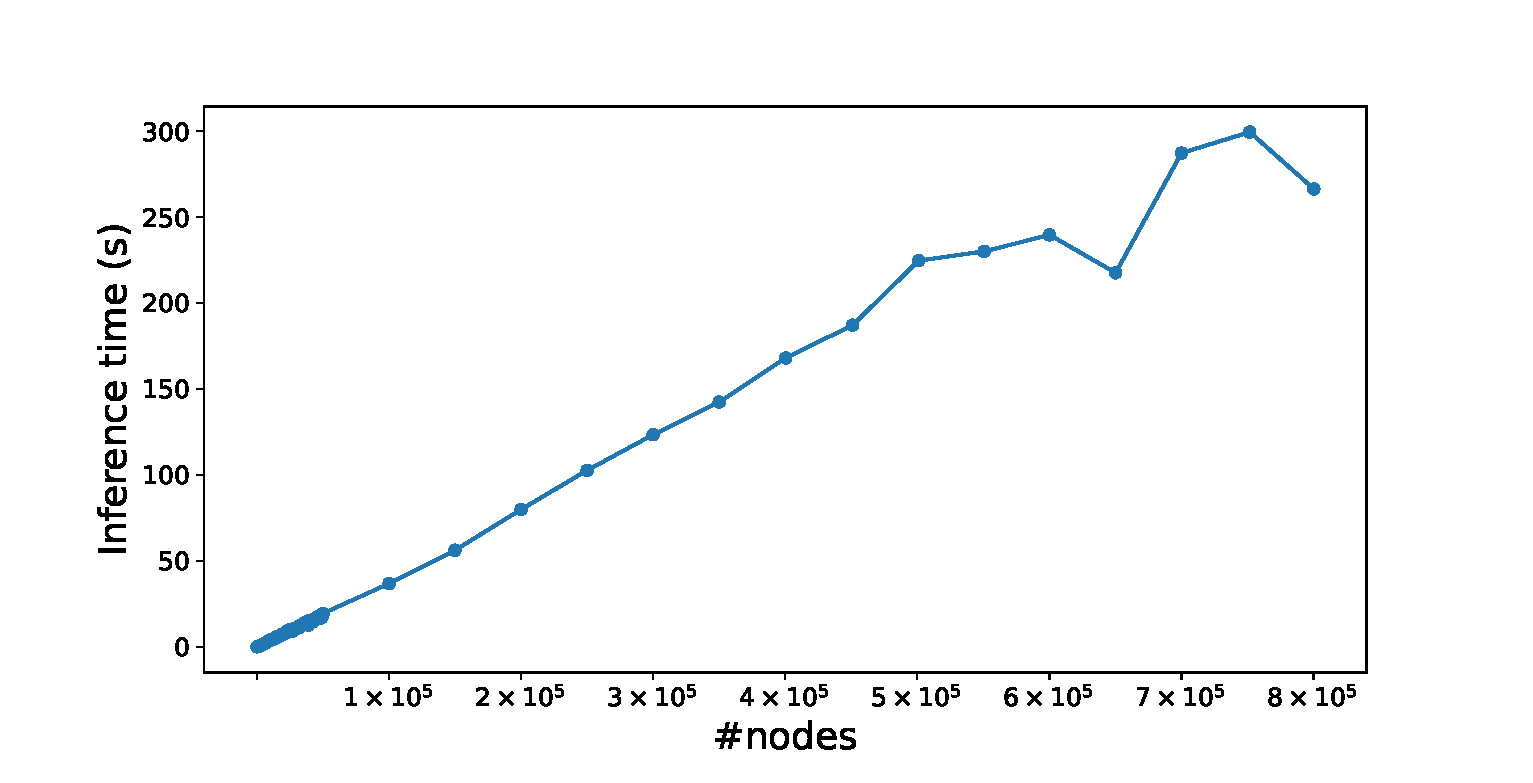
\includegraphics[width=\linewidth]{images/gnn-inference-time.eps}
    \caption{Inference time against the graph network model in seconds on a 48 core Intel Xeon (Skylake) 8168 (2.7GHz) CPU, for increasing graph sizes (excluding input and output processing). The largest problem size for which inference succeeded had 800,445 nodes and 49,609,863 edges. Larger problems ran out of memory (using in excess of 391GiB of RAM)}
    \label{fig:small-runtime-inference}
\end{figure}

While the runtime is already problematic, a bigger problem is the memory usage of this network. In the default implementation, modest compute nodes with only 16GB of RAM (or smaller GPUs) run out of memory at inputs of about $20,000$ nodes. The largest matrix we were able to use as input ($800,000$ nodes) on a more powerful compute node used approximately 400GB of RAM to perform the query.

As with run-time, the memory required for inference in this network also grows linearly with the size of the network. Specifically, for the message passing layers we look to a result in Wu~\cite{wu2020comprehensive}  which demonstrates the memory complexity for graph convolutional layers as $O(Knd + Kd^2)$, with $K$ the number of layers in the network, $n$ the number of nodes and $d$ a fixed constant denoting the size of the hidden features. However, since the network architecture in~\cite{Luz2020} also \textit{concatenates} outputs of each message passing layer as inputs to the next layer, this size of the latent space grows with each layer, with each edge feature consisting of 384 \texttt{float64}'s after the last message passing layer! Luz \etal perform an ablation study which shows that omitting this concatenation slightly hurts the accuracy of the network. 

Memory usage for exact inference in Graph Neural Networks today is known to be problematic~\cite{wu2020comprehensive}. Intermediate layers store the values for all nodes, making memory usage highly sensitive to the size of input graphs. The typical approach is to resort to stochastic sampling of a limited number of nodes or edges in a neighborhood~\cite{graphsage}, but our problem setting for predicting $P$ makes this impossible (we need the edge values of all elements of $P$ in our output). For exact inference against large networks on GPUs, it is possible to loop over the nodes and edges per layer in batches, and copy intermediate layer values back to CPU memory. But this approach requires a manual, device-specific implementation that reduces portability~\cite{inference-against-large-graphs}, and still assumes that the data fits in CPU memory.  

Our situation is not unusual: we see other recent works reporting out-of-memory errors (OOMs) on modest network sizes (e.g. the performance comparison of various frameworks in~\cite{DGL}), and note that benchmarks for GNNs typically use small ($<20,000$ node) problem sizes, focus on training times and report single-node inference~\cite{dwivedi2020benchmarking}~\cite{Wu2021}. This unrepresentative state of affairs is being addressed by initiatives such as the recent Open Graph Benchmark dataset~\cite{hu2020open}.

%\footnote{A notable exception is that large datasets and billions-of-nodes graphs are reported in work for learning Knowledge Graph Embeddings, such as in the papers describing graph embedding frameworks GraphVite~\cite{graphvite} and  PyTorch-BigGraph~\cite{pytorch-biggraph}.}

Of course, we can use further tricks to squeeze more performance from a single node, such as using mixed precision (\texttt{float32} accumulation and \texttt{float16} weights in the network) or reduced precision datatypes for the intermediate vectors instead of the \texttt{float64} widths used by Luz \etal (although we note that these are not supported by the versions of the frameworks used in their original implementation), and possibly reducing the dimensionality of the latent space (not tested in the authors' ablation study). Skillful application of techniques such as inducing sparsity in the model through pruning, and the use of a DL compiler such as TVM \cite{TVM} may reduce the computation and memory usage to allow for much larger single-node inferences. In addition, alternative frameworks like DGL have much better memory use owing to their use of fused message passing kernels that do not store the intermediate message values~\cite{DGL}. However, even with such mitigations, scaling to the large problem sizes with billions of nodes as required by industrial-scale problems is not feasible on a single inference node. 

\paragraph{Distributed inference}
Industrial use cases involving billion-scale graphs, such as that reported by Ying \etal~\cite{Ying_2018} on 18-billion edge graphs at Pinterest, have led to the development of large-scale frameworks.
A survey of leading GNN frameworks (PyTorch Geometric~\cite{pytorch-geometric}, DGL~\cite{DGL}, GraphNets~\cite{battaglia2018relational}, Spektral~\cite{grattarola2021graph}, Angel~\cite{angel}, Graph-Learn~\cite{yang2019aligraph}) shows widespread support for distributed \textit{training}, especially using data-parallel rather then model-parallel techniques, but distributed \textit{inference} (where a single large input graph is distributed over many nodes) remains poorly supported. Our survey found support for distributed inference in recent versions of DGL, Angel, and Graph-Learn but the heavyweight process for initializing the servers and workers, determining graph partitions, and loading the distributed data efficiently (from shared storage) to build the distributed graph is overkill given that we only need to make a single inference during the AMG problem setup phase per multigrid level. We have not re-implemented the model in these frameworks as part of our work.
 

\paragraph{Model input and output processing}
In our integrations with scalable solvers such as HYPRE, we face the problem that the large sparse matrix $A$ is partitioned over distributed compute nodes' memories. The transformation from this sparse matrix into a single ``GraphsTuple'' input for inference against the model using some standard serving framework can easily be implemented in a parallel, distributed fashion, but the interface between this distributed representation and the model framework is awkward: when using a serving framework, e.g. by initiating a request using the gRPC framework, we still need to send the whole graph, and by implication have gathered it into a single originating node's memory. Similarly, the response must be unmarshalled, the sparsity pattern of $P$ re-imposed, and the resulting elements of $P$ repartitioned to their distributed locations to continue with solver setup.

\paragraph{Testing small-graph generalization without retraining}
Despite training on a limited class of matrices that allow for cheap evaluation of the loss function, Luz \etal show some generalization capability of this network to other distributions and even different PDEs problems without retraining, including to a simple 2D FEM problem.

However, we note that the inputs to the network are also shaped by the coarsening strategies and interpolation methods used (they are used in the pre-processing and post-processing stages to impose a sparsity pattern). The authors of~\cite{Luz2020} choose classical Ruge-St\"uben direct interpolation with the CLJP~\cite{cleary1998coarse} coarsening and no Krylov acceleration as their baseline -- a choice which sets the bar for comparison quite low (it produces many more iterations and deeper hierarchies than a more aggressive coarsening and longer-range interpolation). 

Classical AMG is designed for Hermitian positive definite matrices, and our FEM simulations are not guaranteed to produce these.  Before testing how well a pre-trained model can generalize to our dataset, it is important to establish whether a baseline (non-ML) classical Ruge-St\"uben solver, as configured with the coarsening and interpolation~\cite{Luz2020} used during training, can solve our systems. As a test, we use those ``velocity projection'' matrices with fewer than 25,000 rows, comprising 1,624 matrices from the dataset. 

The solver is configured as in~\cite{Luz2020} to perform V-cycles using CLJP coarsening, a classical algebraic strength metric with $\theta=0.25$, a single symmetric sweep of Gauss-Seidel pre- and post-smoothing, and a limit of 12 on the maximum number of levels. With this solver configuration, only 69.2\% of the linear systems in the sampled dataset converge in under 500 iterations. Better results can be expected by using other options, such as smoothed aggregation coarsening with GMRES acceleration. 

%Actually considering only those matrice <25000 we have 
% 2021-06-08 19:17:33,211 - MODEL - INFO - Num model conv: 287 of 1624 = 
% 2021-06-08 19:17:33,211 - MODEL - INFO - Num baseline conv: 1124 of 1624
% 2021-06-08 19:17:33,211 - MODEL - INFO - Num baseline conv not model: 837 of 3646
% 2021-06-08 19:17:33,211 - MODEL - INFO - Num model conv not baseline: 0 of 3646
% 2021-06-08 19:17:33,211 - MODEL - INFO - Num model beat baseline: 13 of 1124
% 2021-06-08 19:17:33,211 - MODEL - INFO - Skipped: 2022 of 3646

In contrast, when using the model from~\cite{Luz2020} to predict values of $P$, we find that only 17.7\% of these systems converge in under 500 iterations. Even in cases where both the model and the baseline converge, the model's predictions result in fewer iterations to convergence only 1.2\% of the time. It has not been able to generalize to the PDE and shapes in our dataset, even for the smallest matrices.







% We note that a baseline (non-ML)  classical Ruge-St\"uben solver is not guaranteed to solve the systems in our dataset (which are not necessarily SPD matrices~\cite{stuben2000algebraic}). To solve systems using our matrices we must use more recent techniques for coarsening (such as PMIS) and longer-range interpolation (such as extended+i), and we only found good convergence when we combined the use of AMG with Krylov acceleration. These choices result in a baseline solver that converges much faster than the baseline in~\cite{Luz2020}, and makes it more difficult for the model to look impressive.



\paragraph{Infeasibility of retraining or fine-tuning with our dataset}
Lastly, we note that the prohibitive cost of evaluating the loss function on large matrices means we cannot use our dataset to retrain or fine-tune the network as it is currently proposed. Since TensorFlow does not currently support sparse inversion of matrices, the large $P^TAP$ matrices must be converted to dense matrices before matrix inversion, for which they are infeasibly large.

% Both approaches preserve the local property, but the second has the opportunity to learn 4-wide.

% Important to note:


% The input distribution is not only determined by the problem geometries and PDE being solved, but also boundary conditions and the sparsity pattern of P and the division of coarse/fine nodes. Re-imposition of sparsity as a post-processing step. One network which generalizes well to different interpolation and coarsening strategies, or loading weights or even new architectures for specialized networks per known coarsening strategy and interpolation strategy? Former requires much more extensive training with a dataset that includes a range of problem geometries, different PDEs with different coefficients 

% TODO: Relatively easy to test this?. Re-train with PMIS and extended interpolation.

% Secondly, the each iteration of AMG involves many more computations than a comparable Krylov such as preconditioned CG, with the result that a pre-conditioned Krylov solver will usually take less time, even if it requires many more iterations. (Although GPU may make AMG more attractive~\cite{}). In fact AMG is often used as a preconditioner: a single iteration of AMG is used to produce an approximation of $A^{-1}$. If we're going to the extra effort of running the ML interpolation, the single iteration has to result in a preconditioner which substantially improves the condition number. Does it?!


% Neither of these criticism take away from the novel achievements in~\cite{Luz2020} and~\cite{Greenfeld2019} that show that ML can be used to learn better operators for AMG -- theirs is clearly pioneering work.

% It is worth stepping back and considering how these models are to be used, from a black box perspective. 

% How often do we need to perform inference against these models? What are our inputs and outputs? How does this fit into the overall program flow.

% During the AMG Setup phase, we must determine the interpolation operator for each level of the hierarchy, where the number of levels in the hierarchy is typically either capped by the user, or is determined by coarsening until the linear system coarsest level can be solved using a direct method: typically at most tens of levels. Each of these need only a single inference against the model. 

% We only do this inference once per level at the start of the solve, and re-use the operator in all subsequent iterations. We only have a 3 solves per timestep, and these will occur separated by relatively long periods of computation. 

% In other words, we will never perform batches of inference for many inputs simultaneously. In each case, the input is a graph representing the entire fine grid. A single, huge input per level.


% \subsection{Results}
% \paragraph{Using our dataset with Luz2020}
% Intriguingly, the authors in~\cite{Luz2020} found that their network, trained on small block-circulant Laplacian matrices with coefficients from a log-normal distribution, could be successfully appliedd to a simple 2D FEM problem without any retraining. 



% Our original intention was to first test how well the network generalised to the large datasets we create. It fails miserably.

% So: how well does it generalise to our matrices?


% Performance of even small is abysmal.
% Memory used when larger,

% Newer versions of Sonnet allow mixed precision training and inference.


% In summary, even ignoring the hoops of training, the compute and memory resources for this small step in the problem setup far exceed those of contemporary non-ML methods and any improvement in the iteration (if any). Wiith this result, we are left to consider the future. 

% How can we do this without calculating SVD on extremely large matrices? ($On^3$)

% Cannot export to ONNX because of custom operators but PyTorch Geomtric Jittable \url{https://github.com/rusty1s/pytorch\_geometric/pull/1191.}

% They did problems up to 400k?!

% Graph\_nets does not support distributed inference where a single graph is distributed among multiple nodes (we note that distributed training is possible, in which case batches of smaller graphs are sharded among workers). DGL does, but even in this case ours is an unusual use case - would normally be sampling only part of the graph.



\section{Conclusion}
To date, the work of Luz, \etal~\cite{Luz2020} remains the only work we are aware of in this domain that works for unstructured grid problems. The proposed model has appealing `black box' properties that mean the solver implementation is separated from the problem discretization, and the model can be used to complement the decades of work optimizing AMG solvers. However, we find that the model (as currently implemented) cannot scale usefully to even moderately sized matrices in our dataset. Although the situation may be improved by more optimization and re-implementation in a more performant framework, single-node inference cannot scale to the billions of nodes required for current applications. Yet unfortunately the current heavyweight setup for distributed graph inference frameworks is not suitable for this problem either: the nature of AMG means that inferences are infrequent (once per level per linear system) and necessarily sequential (cannot be batched for all the levels).  But our work with the proposal from Greenfeld \etal shows that there may be hope for simpler models to achieve good results on these problems, and these simpler networks are currently more amenable to deployment for inference in a distributed setting.

Computation for the coarsening and the classical interpolation must be carried out \textit{in addition} and strictly prior to invoking the ML methods we considered, i.e. the run-time for the setup phase is guaranteed to be substantially longer.  This only pays off if the cost of the additional inferences is recovered by run-time savings from substantially fewer iterations. For the small subset of our dataset with reasonable run-times, this was not the case. 

Our hope had been to extend this approach to testing some of the very large models we are considering (with billions of degrees of freedom), but given the limitations of scaling the Graph Neural Network approach with existing implementations, we terminated our investigation early. Future work is required before these methods are ready for general application to real-world problems.

\paragraph{Future Work}
We are investigating the use of DLPack~\cite{dlpack}, a proposal for an in-memory tensor structure that allows no-copy tensor sharing between DL networks. It already has support in PyTorch, TensorFlow, DGL and PetSc, potentially enabling easier integration of traditional HPC and DL tools.

Re-implementing the model of Luz \etal in a more actively developed framework such as DGL will allow more scope for optimization using techniques such as reduced precision and weight quantization, and can allow evaluating whether stochastic neighborhood sampling can be made to work with this problem and relieve memory pressure.

Adapting the model in~\cite{Luz2020} for smoothed aggregation and longer-range interpolation, and perhaps combining it with preconditioners for FEM such as AMGe~\cite{brezina2001algebraic}, may prove to be more successful for the problems in our dataset. 

Lastly, we are considering a hybrid of the approaches in \cite{Greenfeld2019} and \cite{Luz2020}, in which the distance-4 neighborhoods for each point are gathered at their distributed nodes and passed to local, simpler graph networks which operate only on the small subgraphs, allowing the GNN approach to scale better.
% \section{TODO}
% \begin{itemize}x  
%     \item don't forget to mention woth with AMG mini-app
% \end{itemize}


\section*{Acknowledgments}
This work was funded by the Engineering and Physical Sciences Research Council (EPSRC) via the Advanced Simulation and Modelling of Virtual Systems (ASiMoV) project, EP/S005072/1.

% BibTeX users please use one of
%\bibliographystyle{spbasic}      % basic style, author-year citations
\bibliographystyle{spmpsci}      % mathematics and physical sciences
% \bibliographystyle{spphys}       % APS-like style for physics
\bibliography{bibliography}

\end{document}
